\chapter{}

\begin{figure}[H]
\hfill
\centering
\begin{subfigure}[h]{0.4\linewidth}
    \centering
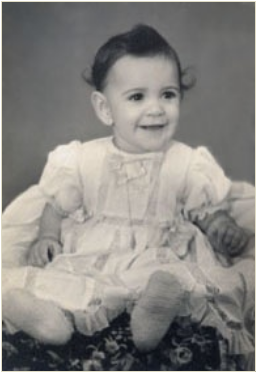
\includegraphics[width=\linewidth]{7/batismo.png}
\caption{Batismo}
\end{subfigure}
\hfill
\begin{subfigure}[h]{0.4\linewidth}
    \centering
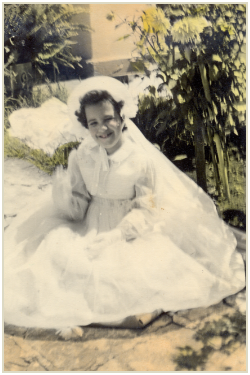
\includegraphics[width=1\linewidth]{7/1a-comunhão.png}
\caption{Primeira Comunhão}
\end{subfigure}
\end{figure}

Fui batizada, crismada, fiz primeira comunhão, novenas, ganhei indulgências, decorei os dez mandamentos, os sete pecados capitais, jurei ser católica apostólica romana e abjurei do demônio ainda em tenra infância, sem ter a menor idéia de quem eram os romanos, os católicos ou o demônio, ou do que fosse pecado. 
Rezava para o Santo Anjo todas as noites e fazia penitência após a confissão. 
Adulta, morei com freiras, trabalhei com padres e casei no religioso. 
Após tudo isso, sou uma católica bissexta que crê firmemente em Deus e muito pouco na Igreja. 
Sou grata a Ele por me ter concedido participação nesse imenso projeto que é a Vida e me inquieta a constatação, nessa altura da minha existência, de que recebi muito mais do que dei. 
Quando leio ou ouço dizer que a Vida não é um dom ou uma graça, mas um caos produzido por uma energia errática e perversa, lembro-me da parábola contada por um jesuíta sobre a formiga que, caminhando com dificuldade sobre uma imensa toalha de renda de fino lavor, bradava contra o desastrado e incompetente artesão que a teceu, maldizendo os buracos onde suas patinhas se enredavam.

Lá pelo meio do meu sexto ano de vida, em sinal de gratidão a Deus pela cura da nefrite que me vitimara, vestiram-me de anjo para acompanhar o pálio de Corpus Christi, numa das muitas procissões que o Vigário da Matriz organizava ao longo do ano. 
Halo dourado cingindo a cabeça, encimado por uma estrela, imensas asas de penas de ganso tingidas, envergando uma camisola longa de tafetá, toda em amarelo radiante, lá fui eu rebocada pela Vó Didi. 

A escolha da cor amarela tinha a ver com o fato de que minha avó era a zeladora do altar de São José, posição de destaque na hierarquia da irmandade do venerável santo, irmandade essa identificada pela fita amarela que suas participantes traziam ao pescoço. 
Na queda de braço entre as tias, irmãs de papai e a avó para decidir de que cor seria o anjo, mamãe optou por dar vitória à D. Didi. 
Talvez porque a cor da fita que identificava a irmandade das tias fosse vermelha. 
Elas pertenciam à irmandade do Sagrado Coração de Jesus, maior e mais importante do que a de São José, pelo menos me parecia, pois a fita que ostentavam era debruada em dourado e o andor que carregavam, sempre maior e mais enfeitado que os outros, saia na parte central da procissão. 

Uma sobrevivência medieval, as irmandades, por ocasião das festas religiosas, assumiam feição de torcidas organizadas em favor deste ou daquele santo padroeiro. Havia a dos Congregados Marianos, para os homens jovens ou solteiros; os mais velhos integravam os Irmãos do Santíssimo e tinham a missão de abrir solenemente as procissões portando grandes tocheiros e envergando uma opa cor de púrpura; as senhoritas casadoiras reuniam-se sob o estandarte das Filhas de Maria, imaculadamente vestidas de branco e ostentando fitas de tafetá azul celeste sobre o peito. 
Ser congregado mariano ou filha de Maria, para as famílias da cidade, era garantia de bom comportamento e pré-requisito de importância no currículo de qualquer jovem postulante ao casamento. 

\begin{figure}[H]
\centering
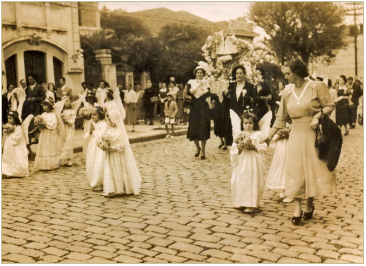
\includegraphics[width=0.8\textwidth]{7/procissão.png}
\caption{Procissão em Araraquara: Tia Angelina, a matriarca dos Ópice, segura a alça esquerda do andor}
\end{figure}

Pois bem, na tal procissão em que eu deveria desfilar de anjo, sabe-se lá por que, o senhor vigário, na última hora, decretou a dissolução da corte celestial e determinou que cada irmandade arcasse com o trabalho de conduzir e vigiar seus querubins. 
Desconfio que não estávamos parecendo suficientemente angelicais aos olhos do velho e cansado sacerdote. 
Ou, talvez, sua escassa paciência tenha se esgotado com a encarniçada disputa entre as representantes das várias facções para decidir se os anjos sairiam por ordem de tamanho, de beleza ou de importância da congregação representada. 

De tudo quanto pode ser reunido sob o rótulo de Religião, lembro-me bem do cheiro que pairava no interior da Matriz, sobretudo nas missas das seis da manhã em que eu acompanhava as tias ou a Vó Didi para me livrar logo da obrigação dominical. 
Era o mesmo cheiro que impregnava o missal, a mantilha e o traje negro de todas elas: uma mistura de flores murchas, cera de vela e um leve odor de mofo misturado à fumaça do incenso do turíbulo que o sonolento coroinha balançava para lá e para cá, hipnotizando meus olhos mal acordados.  
E de um silêncio de mistério que enchia a nave mal iluminada pela primeira claridade da manhã, docemente quebrado pelo cicio dos lábios murchos das velhas beatas no afã de acompanhar o monótono latinório do velho pároco, ainda mais incompreensível porque rouco, baixo e apressado. 
De tempos em tempos, o tilintar da campainha que o coroinha sacudia, reagindo a um cutucão do padre, alertava para a aproximação da parte principal da missa, a comunhão, à qual se seguiria, pouco depois, o esperado ``Ite missa est!''.

A Igreja Matriz da cidade era pequena, mas bem proporcionada. 
No seu interior, como era moda na época, pinturas de \textit{``trompe l’oeil''} imitavam volutas, sancas e florões e anjos e santos habitavam céus azuis cravejados de estrelinhas douradas. 
As paredes exibiam painéis e colunas fingindo mármores preciosos de Carrara. 
O altar-mor era de madeira torneada, pintado de branco e azul e debruado em dourado. 
Uma decoração, enfim, toda compatível com o Olimpo cristão constelado no imaginário popular. 
Tinha lá sua graça.
Um dia, apresentou-se na missa das dez, a mais importante, o clérigo que vinha para finalmente substituir o nosso já muito adoentado vigário, Padre Colturato. 
Bonitão, moderno, bom orador, Padre Orlando chegou causando \textit{``frisson''}. 
E implicando de saída com a velha igreja. 
Araraquara merecia coisa muito melhor, bradou ele do púlpito. 
E logo deu início a campanhas, quermesses e promoções para arrecadação de fundos. Seria uma construção monumental, digna da fé do rebanho araraquarense. 
As opiniões dividiam-se pró e contra a modernização da Matriz. Mas a oratória do novo vigário e o trabalho incessante dos cupins venceram a parada. 
A Matriz seria derrubada. 
A decisão veio a público no final da Quaresma, um pouco antes da Semana Santa.

Na Sexta-Feira, dia em que se dava o ápice das comemorações do período, acontecia o Encontro, evento noturno em que duas procissões iluminadas por velas e partindo de pontos opostos da cidade traziam até o Largo da Câmara, uma, a imagem de Jesus morto em seu ataúde, e outra, a de Nossa Senhora das Dores, com seu manto roxo, suas lágrimas de sangue e o punhal de prata cravado no peito. 
E o rosto emoldurado pelos cachos da Tia Angelina, a matriarca dos Ópice, que os havia cortado e doado à santa no cumprimento de uma promessa. 
Eu torcia sempre para que meus pais escolhessem acompanhar a primeira procissão, porque nela ia a Verônica, uma mulher oculta em longo e negro véu, que em cada esquina do trajeto subia num banquinho e, entoando um canto pungente, desenrolava um pano branco onde se via impresso o rosto martirizado do Cristo. 
Nela iam ainda as matracas, instrumentos medievais que serviam para alertar para a aproximação do féretro, feitos de uma aldrava de metal que batia contra uma prancha de madeira, produzindo um som cavo de ossos chacoalhando. Aquela encenação carregada de dramaticidade, à luz oscilante das velas, estampava na fisionomia das pessoas qualquer coisa de fantasmagórico. Até as feições do pessoal de casa me pareciam sobrenaturais. 
A impressão era tamanha que ainda sou capaz de ouvir as vozes misturadas de homens e mulheres cantando e implorando: \textit{``Pela Virgem Dolorosa, Nossa Mãe tão piedosa, perdoai, ó meu Jesus; perdoai, ó meu Jesus!''}.

Pois bem, naquela sexta-feira, após o encontro e incorporadas, as duas procissões seguiram para o desfecho na Igreja Matriz, onde acontecia a Hora de Guarda, cerimônia em que a imagem do corpo do Senhor era velada pelos fiéis até o alvorecer da Aleluia. 
Ia o culto a meio, quando um estrondo de fim de mundo rasgou o céu e um aguaceiro daqueles desabou. 
Entretido na procissão, o povo não se deu conta da tempestade que se aproximava. 
O vento invadiu a nave sibilando, sacudindo e batendo portas e janelas. 
O grande lustre que pendia da cúpula da Igreja desandou num balanço alucinado e acabou despencando, acompanhado de um dos vitrais que, após violento estalo, veio igualmente estilhaçar-se no chão. 
À chuva de cacos seguiu-se uma torrente de água que inundou tudo. 
Espavorida, a multidão arremeteu para as saídas, esquecendo-se do morto sagrado que lá ficou com sua Santa Mãe entre os escombros. 
Corremos nós também, rua abaixo, protegidos apenas pelos \textit{``Santa Clara!''} que a minha mãe invocava entre sinais da cruz, a cada vez que um raio explodia sobre nossas cabeças. 
Chegamos em casa molhados dos cabelos aos sapatos. 
A tempo de descobrir que parte do nosso telhado jazia espatifado sobre a calçada e generosas goteiras, caindo através do forro de madeira, haviam transformado nossos quartos em lagoas. 
Dormimos papai, mamãe, Reginaldo e eu amontoados num pedaço da sala que se conservara seco.

Por muito tempo, Padre Orlando teve que ouvir que aquela Sexta-Feira Santa tinha sido o castigo merecido pela nefasta decisão de derrubar a velha Matriz. 
Verdade ou não, o fato é que o pretensioso projeto que aos poucos foi se materializando no lugar da humilde igrejinha nunca foi terminado. 
O solo poroso não lhe suportou o peso e a construção rachou ameaçadoramente quando o trabalho ainda nem chegara à metade. 
E até hoje ela lá está, inacabada, grandalhona e deforme como se mutilada por uma praga. 
\textit{``-- Monumento à arrogância daquele padre de meia-tigela''}, esconjurou minha mãe até o fim da vida. 
O desprezo veio se somar à aversão quando ela soube, poucos meses depois, que a reverendíssima figura tinha abandonado a batina e fugido com a bela filha do confeiteiro.

Adulta, trabalhei com jesuítas. Revisitei lembranças, cauterizei feridas que o desencanto abriu na minha claudicante fé, fortaleci algumas intuições apenas pressentidas anteriormente, mas também vi evaporar outras que até então me traziam consolo. Aí comecei uma lenta e difícil jornada de descoberta de um caminho para um Deus que eu pressinto, não alcanço e pelo qual anseio, como todos os outros, mesmo aqueles que O desacreditam.  Ensinou um rabino que, para negar Deus, é preciso que haja um Deus a ser negado. É preciso descobrir de que Deus somos ateus. E encontrar o Deus verdadeiro que, dizem, aguarda-nos lá onde nos é mais difícil procurá-lo: no mais profundo de nós mesmos. 